%\pdfoutput=1

\documentclass[10pt,journal]{IEEEtran}

\usepackage{amsmath}
\usepackage{amssymb}
\usepackage{amsthm}
\usepackage{algorithm}
%\usepackage{algorithmic}
%\usepackage{fullpage}
\usepackage{tikz}
\usepackage{xifthen}
\usepackage{tabu}
\usepackage{graphics}
\usepackage{subfig}
\usepackage{epstopdf}
\usepackage{epsfig}
\usepackage{caption}
\usepackage{float}
\usepackage{pgfplotstable}
\usepackage{pgfplots}
%\usepackage[utf8]{inputenc}
%\numberwithin{equation}{section}  
\newtheorem{theorem}{Theorem}%[section]           %[section]   %numberes automatically
\newtheorem{lemma}[theorem]{Lemma}         %[theorem] 
\newtheorem{corollary}[theorem]{Corollary}     %{corollary}{Corollary}[theorem]   
\newtheorem{proposition}[theorem]{Proposition}
\newtheorem{claim}[theorem]{Claim}
\newtheorem{ass}[theorem]{Assumption}
\newtheorem{fact}[theorem]{Fact}
\newtheorem{heuristic}[theorem]{Heuristic}
\newtheorem{definition}[theorem]{Definition}
\newtheorem{assumption}[theorem]{Assumption}
\newtheorem{remark}[theorem]{Remark}
\newtheorem{exmp}[theorem]{Example}   
\newcommand{\new}[1]{\textcolor{red}{#1}}

\newcommand{\red}[1]{\textcolor{red}{#1}}
\newcommand{\blue}[1]{\textcolor{blue}{#1}}


\def\x{{\mathbf x}}
\def\R{{\mathbb{R}}}
\def\E{{\mathbb{E}}}
\def\L{{\cal L}}
\def\lin{\text{lin}}
\newcommand{\norm}[1]{\|#1\|}
\def\rank{\text{rank}}
\def\O{{\mathcal{O}}}
\def\P{{\mathcal{P}}}
\def\pr{\mathbb{P}}
\def\la{\lambda}
\def\A{\mathcal{A}}
\def\T{\widetilde}
\def\Ta{{\mathcal{T}}}
\def\H{{\mathcal{H}}}
\def\M{\mathcal{M}}
\def\U{\mathbb{U}}
\def\n{\Big{\|}}
\def\1{\mathbf{1}}     
\def\layersep{2.5cm}
\usepackage{enumitem}

\usepackage{todonotes}
\def\poly{\text{poly}}
\def\Tr{\text{Tr}}

\setlength{\textfloatsep}{14pt plus 1.0pt minus 1.0pt}
%\usepackage{authblk}
%\usepackage[margin=1in]{geometry}
%\usepackage[parfill]{parskip}
%\usepackage{times}
%\usepackage{graphicx}


%\usepackage{natbib}
%\usepackage{float}
\usepackage{algpseudocode}
%\usepackage{rotating}

\usepackage{amsfonts}
\usepackage{mathtools}
\usepackage{hyperref}
\newcommand{\theHalgorithm}{\arabic{algorithm}}
%\usepackage[shortcuts]{extdash}
\newcommand{\SREC}{S\=/REC}
\DeclareMathOperator*{\argmin}{arg\,min}
\DeclareMathOperator*{\argmax}{arg\,max}
\def\R{{\mathbb{R}}}
%\newtheorem{theorem}{Theorem}[section]
\newcommand{\mb}[1]{\mathbf{#1}}
%\newtheoremstyle{exampstyle}
%  {10pt} % Space above
%  {10pt} % Space below
%  {} % Body font
%  {} % Indent amount
%  {\bfseries} % Theorem head font
%  {.} % Punctuation after theorem head
%  {.5em} % Space after theorem head
%  {} % Theorem head spec (can be left empty, meaning `normal')
%\theoremstyle{exampstyle} \newtheorem{theorem}{Theorem}[section]
%
%\newtheorem{corollary}{Corollary}[theorem]
%\newtheorem{lemma}[theorem]{Lemma}
%\newtheorem{definition}{Definition}
%\title{Compressed Sensing on GANs using Iterative Projections}

\def\sgn{\mathrm{sgn}}
\def\card{\mathrm{card}}
\def\t{\intercal}
\def\t{\top}
\def\cosamp{\mathrm{CoSaMP}}
%\author{Viraj Shah}
%\author{Chinmay Hegde}
%\affil{ECpE Department, Iowa State University}

%\newcommand{\norm}[1]{\|#1\|}
\newcommand{\eps}{\epsilon}
\newcommand{\wh}[1]{\widehat{#1}}
\newcommand{\s}{0.18}
\usepackage{hyperref}
\usepackage[utf8]{inputenc}
\usepackage{booktabs}
\usetikzlibrary{calc}
\hyphenation{op-tical net-works semi-conduc-tor}
\begin{document}
\title{Reconstruction from Modulo Measurements}

\author{
	Viraj Shah and Chinmay Hegde \\
	Electrical and Computer Engineering Department \\
	Iowa State University \\
	Ames, IA, USA 50010
	\thanks{Email: \{viraj,chinmay@iastate.edu\}. This work was supported by grants CCF-1566281 and CAREER CCF-1750920 from the National Science Foundation, and a faculty fellowship from the Black and Veatch Foundation, and a GPU grant from the NVIDIA Corporation.
	}
	%  \texttt{viraj,chinmay@iastate.edu} \\
}


\maketitle

\begin{abstract}
	We consider the problem of recovering a signal from its compressed modulo measurements.
\end{abstract}
\section{Introduction}
\label{sec:intro}
\subsection{Motivation}
The problem of recovering a signal (or image) from its nonlinear observations is widely encountered in the domain of signal processing, signal acquisition and imaging systems. One such example is the classical problem of phase retrieval, which arises in numerous imaging applications including ptychography, diffraction imaging and astronomical imaging. In such imaging systems, due to the limitations of the optical sensors, only the magnitude of the light rays can be measured but not the phase. As each linear observation losses its phase, the effective forward model can be expressed as a composition of nonlinear absolute value function with the linear observation function. Though the phase retrieval problem is challenging ill-posed inverse problem, it is well-studied in the literature and there exists multiple provably efficient algorithmic procedures to solve it in different settings. \cite{}\todo{cite}

Most of the image and signal acquisition systems suffer from the problem of limited dynamic range. It is well known that real signals contain a large range of intensity levels, and not all of them can be accurately captured due to hardware limited dynamic range of conventional acquisition systems. If tuned incorrectly, most intensity levels can lie in the saturation region of the sensors, causing loss of information through clipping of signals. The problem gets amplified in the case of multiplexed imaging systems, where required dynamic range is very high because of the fact that the observed signal intensity is a sum of various weighted versions of the original signal. The obvious solution to this issue is to increase the dynamic range of the sensors, but unfortunately it is not always possible due to expensive hardware. An alternative approach is the deploy a specifically designed sensors named modulo sensors. As the name suggests, such sensor wraps the observed signal intensity value over given dynamic range, which is analogous to familiar modulo operation with respect to parameter $R$. Usage of the modulo sensor to capture the linear measurements adds an additional effect of modulo operation over each observation, making the forward model highly nonlinear. Recovery of the underlying signal from such modulo measurements turns out to be a challenging and significant yet rarely studied problem in the domain of signal and image processing. 

For most of the nonlinear inverse problems that were solved in the literature, such results require overcomplete obervations, meaning the number of minimum measurements $m$ require for the signal recovery is higher than the ambient dimension $n$ of the signal itself. For the cases where $m$ and $n$ are large, this requirement puts limitation on computation and storage of the measurements. Thus, in this paper, we focus on solving the problem of modulo recovery with very few number of samples. This can be achieved by assuming that the underlying signal obeys a certain low-dimensional structure. Typically, sparsity in some known basis is used as a structural assumption in many imaging applications as many real signals are known to be sparse in some basis. 

\todo{some drawbacks of the prior work, advantages of our work over others}
\subsection{Setup}
\label{subsec:setup}
We formalize the above discussion as follows. Assume $\mathcal{X} \subseteq \R^n$ to be a given (known) subset in the data space, and consider a signal (or image) $\mb{x}^* \in \mathcal{X}$. We construct $\mathbf{A} = \left[\mathbf{a_1~a_2~...~a_m}\right]^T$ with i.i.d. Gaussian entries. We aim to recover the original signal $\mb{x^*}\in \R^n$ from its compressed modulo measurements $y_i$ defined as:
\begin{equation}
y_i=\mod(\langle \mathbf{a_i} \cdot \mathbf{x^*} \rangle,R)~\textnormal{for}~i = \{1,2,...,m\},
\label{eq:modmeas1}
\end{equation} 
where $\mod(\cdot)$ is modulo operation with respect to a fixed, real-valued parameter $R$. We set $m<n$. For simplicity, we assume that the modulo function operates only within two periods, one each on the either side of the origin, as shown in the Fig.~\ref{fig:modop}. The primary assumption in our model is that the natural signal $\mathbf{x^*}$ is $s-$sparse in a chosen basis. 

\begin{figure}[h]
	\begin{center}
		\begin{tikzpicture}[scale=0.7, every node/.style={scale=0.7}]
		\draw[<->] (-4,0) -- (4,0) node[right] {$t$};
		\draw[->] (0,-1) -- (0,4) node[above] {$f(t)$};
		\draw[scale=0.5, dashed, thick] (0,4)--(7,4) node[right]{$R$};
		\draw (1.5,-0.5) node(below) {$p_i = 0$};
		\draw (-1.5,-0.5) node(below) {$p_i = 1$};
		\draw (0,-1.5) node(right) {$f(t) = \mod(t,R)$};
		\draw[scale=0.5,domain=-7:0,smooth,variable=\x,cyan, ultra thick] plot ({\x},{\x+4});
		\draw[scale=0.5,domain=0:7,smooth,variable=\x,cyan, ultra thick]  plot ({\x},{\x});
		\end{tikzpicture}
	\end{center}
	\caption{\emph{Modified modulo function for the given problem}}
	\label{fig:modop}
\end{figure}

\subsection{Our contributions}
The key contribution of our approach is to identify and draw parallels between the problems of phase retrieval and modulo recovery, which allowed us to bring in the ideas from the classical phase retrieval solutions into relatively new setup of modulo recovery problems.
\subsection{Techniques}
The proposed MoRAM algorithm is conceptually simple yet novel step in the direction of solving the problem of modulo recovery. Our work takes a fresh approach for solving the modulo recovery problem by borrowing the ideas from the well studied field of phase retrieval and compressive sensing - which has been done for the first time to the best of our knowledge. The commonality that we identified in these two different class of problems is the need of undoing the effect of a piecewise linear function in both the cases. While we deal with the modified version of modulo function with two periods in the case of modulo recovery, phase retrieval deals with undoing the effect of absolute value function which is piece wise linear too. 
At the same time, difference between the behavior of both the functions is also evident, which restricts us from using the phase retrieval solutions as it is for solving modulo recovery problem. Fig.~\ref{fig:compare} compares the behavior of both the modulo ($f(t)$) and absolute value ($g(t)$) functions. Both the functions are identical in the positive half, but differs significantly in the negative half. For negative inputs, 

\begin{figure}[h]
	\begin{center}
		\begin{tikzpicture}[scale=0.7, every node/.style={scale=0.7}]
		\draw[<->] (-4,0) -- (4,0) node[right] {$t$};
		\draw[->] (0,-1) -- (0,4);
		\draw[scale=0.5, dashed, thick] (0,4)--(7,4) node[right]{$R$};
		\draw (1.5,-0.5) node(below) {$p_i = 0$};
		\draw (-1.5,-0.5) node(below) {$p_i = 1$};
		\draw[scale=0.5,cyan,ultra thick] (1.5,6.5)--(2.5,6.5) node[right,black]{$f(t)$};
		\draw[scale=0.5,dotted,red,ultra thick] (1.5,5.5)--(2.5,5.5) node[right,black]{$g(t)$};
		\draw (0,-1.5) node(right) {$f(t) = \mod(t,R),~g(t)=\mathrm{abs}(t)$};
		\draw[scale=0.5,domain=-7:0,smooth,variable=\x,cyan, ultra thick] plot ({\x},{\x+4});
		\draw[scale=0.5,domain=0:7,smooth,variable=\x,cyan, ultra thick]  plot ({\x},{\x});
		\draw[scale=0.5,domain=0:7,smooth,variable=\x,red, ultra thick, dotted]  plot ({\x},{\x});
		\draw[scale=0.5,domain=-7:0,smooth,variable=\x,red, ultra thick, dotted]  plot ({\x},{-\x});
		\end{tikzpicture}
	\end{center}
	\caption{\emph{Comparision between modulo function ($f(t) = \mod(t,R)$); and absolute value function ($g(t) = \mathrm{abs}(t)$)}}
	\label{fig:compare}
\end{figure}

\subsection{Paper organization}
The reminder of the paper is organized as follows. In section~\ref{sec:prior}, we briefly discuss the prior work. Sections~\ref{sec:prelim} contains notation and mathematical model used for our analysis. In section~\ref{sec:algo}, we introduce the MoRAM algorithm, and provide a theoretical analysis of its performance. We demonstrate the performance of our algorithm by providing series of numerical experiments in section~\ref{sec:exp}. Section~\ref{sec:disc} provides concluding remarks.
\section{Prior work}
\label{sec:prior}

\emph{\textbf{Phase retrieval:}} Approaches to solve phase retrieval problem can be broadly classified into two categories: convex and non-convex. 
Convex approach usually consist of solving a constraint optimization problem after linearizing the problem. PhaseLift algorithm \cite{candes2013phaselift} and its variations \cite{gross2017improved}, \cite{candes2015phasediff} come under this category. Typical non-convex approaches involve finding a good initialization followed by iterative minimization, \textit{e.g.} Approaches based on Amplitude flow \cite{wang2016sparse,wang2016solving} and Wirtinger flow \cite{candes2015phase, zhang2016reshaped,  chen2015solving, cai2016optimal}.

In recent works, phase retrieval problem for the cases where underlying signal is sparse is of growing interest. Some of the convex approaches for sparse phase retrieval includes \cite{ohlsson2012cprl, li2013sparse,bahmani2015efficient,jaganathan2012recovery}. Similarly, non-convex approaches for sparse phase retrieval includes \cite{netrapalli2013phase, cai2016optimal, wang2016sparse}. Our approach in this paper towards solving the modulo recovery problem is mainly inspired from the non-convex sparse phase retrieval framework advocated in \cite{Jagatap2017}. 

\emph{\textbf{Modulo recovery:}} The modulo recovery problem is also known in the literature
as phase unwrapping. The algorithm proposed in \cite{bioucas2007phase} is specialized to images, and employs graph cuts for phase unwrapping from a single modulo measurement per pixel. However, the inherent assumption that the input image has very few sharp discontinuities makes it unsuitable for practical situations with textured images. Our main motivation for this paper is the work of \cite{ICCP15_Zhao} on HDR imaging using a modulo camera sensor. It proposes multi-shot UHDR algorithm for image reconstruction using multiple measurements. The more robust version of it is further proposed in \cite{Lang2017}. However, both these methods depend on carefully decided camera exposures and don't include sparsity in their models. In our previous work \cite{Shah}, we proposed an algorithm based on \cite{ICCP15_Zhao, soltani2017stable} for signal recovery from quantized modulo measurements, which can also be adapted for sparse measurements. 

Given the modulo samples of a bandlimited function, \cite{Bhandari} provides a stable algorithm for perfect recovery of the signal and also proves sufficiency conditions that guarantees the perfect recovery. \cite{Cucuringu2017} formulates and solves an QCQP problem with non-convex constraints for recovering the correct samples of the unknown function from its modulo 1 ($R =1$) samples. However, both these methods relay on the smoothness of the bandlimited function as a prior structure on the signal, and can't be used in our setup.

\section{Preliminaries}
\label{sec:prelim}
\subsection{Notation}
\label{subsec:nota}
In this section, we introduce the notation used throughout in the paper. We denote matrices using bold capital-case letters ($\mb{A,B}$), column vectors using bold-small case letters ($\mb{x,y,z}$ etc.) and scalars using non-bold letters ($R,m$ etc.). Letters $C$ and $c$ are used to represent constants that are large enough and small enough respectively. We use $\mb{x}^\t,\mb{A}^\t$ to denote the transpose of the vector $\mb{x}$ and matrix $\mb{A}$ respectively. The cardinality of set $S$ is expressed using the operator $\card(S)$.

We define the signum function as $\sgn(x) := \frac{x}{|x|}$ for every $x \in \R, x \neq 0$, with the convention that $\sgn(0)=1$.
An $i^{th}$ element of the vector $\mb{x} \in \R^n$ is denoted by $x_{i}$. Similarly, $i^{th}$ row of the matrix $\mb{A} \in \R^{m \times n}$ is denoted by $\mb{a_i}$, while the element of $\mb{A}$ in $i^{th}$ row and $j^{th}$ column is denoted as $a_{ij}$. The projection of vector $\mb{x} \in \R^n$ onto a set of coordinates $S$ is represented as $\mb{x}_S \in \R^n,~\mb{x}_{S_j} = \mb{x}_j$ for $j \in S$, and $0$ elsewhere. 

%Projection of matrix $\mb{M} \in \R^{m\times n}$ onto $S$ is $\mb{M}_S \in \R^{m\times n},~\mb{M}_{S_{ij}} = \mb{M}_{ij}$ for $i, j \in S$, and $0$ elsewhere.

\subsection{Mathematical model}
\label{subsec:model}
As depicted in Fig.~\ref{fig:compare}(a), we consider the modulo operation within 2 periods (one in the positive half and one in the negative half). We assume  that the value of dynamic range parameter $R$ is large enough so that all the measurements $\langle \mathbf{a_i} \cdot \mathbf{x^*} \rangle$ are covered within the domain of operation of modulo function. In terms of a signum function, modulo function under consideration can be defined as, 
$$
f(t) :=\mod(t,R) = t+\left( \frac{1-\sgn(t)}{2}\right)R.
$$
One can easily notice that the modulo operation in this case is nothing but an addition of scalar $R$ if the input is negative, while the non-negative inputs remain unaffected by it. If we divide the number line in these two bins, then the coefficient of $R$ in above equation can be seen as a bin-index, a binary variable which takes value $0$ when $\sgn(t)=1$, or $1$ when $\sgn(t)=-1$.

Inserting the definition of modulo operation in measurement model of Eq.~\ref{eq:modmeas0} gives,
\begin{equation}
y_i= \langle \mathbf{a_i} \cdot \mathbf{x^*} \rangle+\left( \frac{1-\sgn(\langle \mathbf{a_i} \cdot \mathbf{x^*} \rangle)}{2}\right)R,~~i = \{1,..,m\}.
\label{eq:modmeas2}
\end{equation} 
Note that in Eq.~\ref{eq:modmeas2}, the coefficient of $R$ is a binary column vector represented as a bin-index vector $\mb{p} \in \R^m$. Each element of the true bin-index vector $\mb{p}^*$ is given as,
$$
p^*_i = \frac{1-\sgn(\langle \mathbf{a_i} \cdot \mathbf{x^*} \rangle)}{2},~~i = \{1,..,m\}.
$$


If we ignore the presence of modulo operation in above formulation, then it reduces to a standard compressive sensing problem. In that case, the compressed measurements $y_{c_i}$ would just be equal to $\langle \mathbf{a_i} \cdot \mathbf{x^*} \rangle$.    %Variety of algorithms are available in literature that can recover the true signal exactly from its compressed measurements. Theoretical recovery guarantees for algorithms such as $\cosamp$ and basis-pursuit are also well-studied. 

While we have access only to the compressed modulo measurements $\mb{y}$, it is useful to write $\mb{y}$ in terms of true compressed measurements $\mb{y}_c$. 

Thus,
$$
y_i = \langle \mathbf{a_i} \cdot \mathbf{x^*} \rangle + p^*_iR = y_{c_i}+p^*_iR.
$$

It is evident that if we can recover $\mathbf{p^*}$ successfully, we can calculate the true compressed measurements $\langle \mathbf{a_i} \cdot \mathbf{x^*} \rangle$ and use them to reconstruct $\mathbf{x^*}$ with any sparse recovery algorithm such as CoSaMP or basis-pursuit.

\section{Mathematical model}
\label{sec:model}
Let us introduce some notation. We denote matrices using bold capital-case letters ($\mb{A,B}$), column vectors using bold-small case letters ($\mb{x,y,z}$ etc.) and scalars using non-bold letters ($R,m$ etc.). %The superscript $\t$ to denotes the transpose. 
The cardinality of set $S$ is given by $\card(S)$. The signum function is defined as $\sgn(x) := \frac{x}{|x|}, \forall x \in \R, x \neq 0$, with $\sgn(0)=1$. %An $i^{th}$ element of the vector $\mb{x} \in \R^n$ is denoted by $x_{i}$.% Similarly, $i^{th}$ row of the matrix $\mb{A} \in \R^{m \times n}$ is denoted by $\mb{a_i}$, while the element of $\mb{A}$ in $i^{th}$ row and $j^{th}$ column is denoted as $a_{ij}$. 
The projection of vector $\mb{x} \in \R^n$ onto a set of coordinates $S$ is represented as $\mb{x}_S \in \R^n,~\mb{x}_{S_j} = \mb{x}_j$ for $j \in S$, and $0$ elsewhere.

As depicted in Fig.~\ref{fig:compare}(a), we consider the modulo operation within 2 periods.
% and assume that the value of dynamic range parameter $R$ is large enough so that all the elements of $\mb{Ax^*}$ are covered within the domain of operation of modulo function.
If we write the modulo function of Fig.~\ref{fig:compare}(a) in terms of a signum function, then the measurement model of Eq.~\ref{eq:modmeas0} becomes, 
\begin{equation}
y_i= \langle \mathbf{a_i} \cdot \mathbf{x^*} \rangle+\left( \frac{1-\sgn(\langle \mathbf{a_i} \cdot \mathbf{x^*} \rangle)}{2}\right)R,~~i = \{1,..,m\}.
\label{eq:modmeas2}
\end{equation} 
If we divide the number line in two bins, then the coefficient of $R$ in above equation can be seen as a bin-index, a binary variable which takes value $0$ when $\sgn(t)=1$, or $1$ when $\sgn(t)=-1$. We denote such bin-index vector as $\mb{p} \in \R^m$. Each element of the true bin-index vector $\mb{p}^*$ is given as,
$$
p^*_i = \frac{1-\sgn(\langle \mathbf{a_i} \cdot \mathbf{x^*} \rangle)}{2},~~i = \{1,..,m\}.
$$

If we ignore the presence of modulo operation in above formulation, then it reduces to a standard compressive sensing problem. In that case, the compressed measurements $y_{c_i}$ would just be equal to $\langle \mathbf{a_i} \cdot \mathbf{x^*} \rangle$. While we have access only to the compressed modulo measurements $\mb{y}$, it is useful to write $\mb{y}$ in terms of true compressed measurements $\mb{y}_c$. Thus,
$$
y_i = \langle \mathbf{a_i} \cdot \mathbf{x^*} \rangle + p^*_iR = y_{c_i}+p^*_iR.
$$

It is evident that if we can recover $\mathbf{p^*}$ successfully, we can calculate the true compressed measurements $\langle \mathbf{a_i} \cdot \mathbf{x^*} \rangle$ and use them to reconstruct $\mathbf{x^*}$ with any sparse recovery algorithm such as CoSaMP~\cite{needell2010cosamp} or basis-pursuit~\cite{chen2001atomic,spgl1:2007,BergFriedlander:2008}.

\section{Algorithm and Main Results}
Given $\mathbf{y, A}, s, R$, our approach recovers $\mathbf{x^*}$ and $\mathbf{p^*}$ in two steps: (i) an initialization step, and (ii) descent step via Alt-Min.

\subsection{Initialization by re-calculating the measurements}
\label{sec:init}	
Similar to other non-convex approaches, MoRAM also requires an initial estimate $\mathbf{{x}^0}$ that is close to the true signal $\mathbf{{x}^*}$.
% We propose a novel initialization method to re-calculate the true Gaussian measurements ($\mb{y_c}= \mb{Ax^*}$) from the available modulo measurements. We undo the effect of modulo operation for the fraction of the total measurements, and calculate the initial estimate using such corrected measurements.

To do so, we first introduce a hyper-parameter $\rho$ that approximates the spread of the entries of $\mathbf{Ax^*}$. We choose a value of $\rho$ such that it bounds the maximum element of $|\mathbf{Ax^*}|$ with very high probability. As shown in Fig.~\ref{fig:densityplot}, with very high probability, $\mathbf{Ax^*}$ lies within $[-\rho, \rho]$. In Fig.~\ref{fig:densityplot} (a) and (b), we provide the density plots of the $\mb{y_c} = \mathbf{Ax^*}$ and $\mb{y} = \mathbf{\mod(\mathbf{Ax^*})}$ respectively. Note that the compressed measurements $\mathbf{y_c}$ follow the standard normal distribution, as $\mb{A}$ is Gaussian random matrix. These plots essentially depict the distribution of our observations before and after the modulo operation.%, and help us to understand the transformation effected by modulo operation. %In practice, $\rho$ can be calculated based on tail bounds.

With reference to Fig.~\ref{fig:densityplot}(a), we divide the compressed observations $\mb{y_c}$ in two sets: $\mb{y_{c,+}}$ contains all the positive observations lying in $[0,\rho]$ with bin-index$=0$ (orange), while $\mb{y_{c,-}}$ contains all the negative ones in $[-\rho,0]$ with bin-index$=1$ (green). Similarly, in Fig.~\ref{fig:densityplot}(b), modulo observations $\mb{y}$ can also be divided in two sets $\mb{y}_+ = \mod(\mb{y}_{c,+})$ and $\mb{y}_- = \mod(\mb{y}_{c,-})$. Modulo function shifts the set $\mb{y}_{c,-}$ to the right by $R$, while leaves the set $\mb{y}_{c,+}$ unaffected. Thus, the sets $\mb{y}_-$ and $\mb{y}_+$ occupy the interval $[R-\rho,R]$ and $[0,\rho]$ respectively. From that, it can be concluded with surety that all the modulo observations lying in the interval $[\rho, R]$ (green) are part of set $\mb{y}_{c,-}$, and have bin-index value equal to $1$. Similarly, all the modulo observations lying in the interval $[0,R-\rho]$ (orange) are part of set $\mb{y}_{c,+}$, and have bin-index value equal to $0$. Nothing can be concluded for other modulo observations lying in $[R-\rho,\rho]$ (gray, region of uncertainty). We assign bin-index$=0$ for such observations. Thus, the corrected bin-index vector can be calculated as:
\begin{equation}
{p}^{init}_{i} = 
\begin{cases}
0,& \text{if } 0\leq y_i < (R-\rho) \\
0,& \text{if } (R-\rho)\leq y_i < \rho ~ \textnormal{(region of uncertainty)} \\
1,& \text{if } \rho \leq y_i < R \\
\end{cases}
\label{eq:rcm}
\end{equation}
%\begin{itemize}
%	\item Only the values lying on the negative side of the x-axis are going to be affected.
%	\item Values lying very close to the origin on the negative side of the x-axis in the first density plot, would now shift by $R$, and would occupy a place very close to $R$ in second plot. For $R>\rho$, this region is shaded with green color in Fig.~\ref{fig:hist2}. Correct bin-index for the elements in $\mathbf{y}$ with value lying between $\rho$ and $R$ is $p^{init}_{i} = 1$.
%	\item For $R>\rho$, density plot of the positive region very close to the origin would remain unaffected. This region is shaded with orange color in Fig.~\ref{fig:hist2}. Correct bin-index for all the elements in $\mathbf{y}$ with value lying between $0$ and $R-\rho$ is $p^{init}_{i} = 0$.
%	\item Nothing can be concluded for measurements lying in between the above mentioned ranges. This region is shaded with gray color in Fig.~\ref{fig:hist2}. Correct bin-index cannot be identified for this region, so we assign all the elements in $\mathbf{y}$ with value lying between $0$ and $(R-\rho)$ as $p^{init}_{i} = 0$. The lower and upper bounds ($t_l$~\&$~t_u$) of this region of uncertainty can be obtained as, 
%	\begin{align*}
%	t_l & = R-\rho, \\
%	t_u & = R.
%	\end{align*}
%	%\item Irrespective of relationship between $\rho$ and $R$, all the values lying in the negative half of the real line have the bin-index equal to $1$, and all the values greater than $R$ have the bin-index equal to $0$.
%\end{itemize}

\begin{algorithm}[t]
	\caption{\textsc{MoRAM-initialization}}
	\label{alg:RCM}
	\begin{algorithmic}
		\State\textbf{Inputs:} $\mathbf{y}$, $\mathbf{A}$, $s$, $R$, $\rho$
		\State\textbf{Output:}  $\mb{x^0}$
		\State $U \leftarrow \emptyset$%, $t_l \leftarrow (R-\rho)$, $t_u \leftarrow R$
		\For {$i= 0:m$}
%		\If {$y_l<0$}
%		\State {$p^{rcm}_l = 1$, $T \leftarrow T \cup {l}$}
%		\ElsIf {$0\leq y_l < t_l$}
%		\State {$p^{rcm}_l = 0$, $T \leftarrow T \cup {l}$}
%		\ElsIf {$t_l\leq y_l < t_u$}
%		\State {$p^{rcm}_l = 0$}
%		\ElsIf {$t_u \leq y_l < R$}
%		\State {$p^{rcm}_l = 1$, $T \leftarrow T \cup {l}$}
%		\ElsIf {$R  \leq y_l$}
%		\State {$p^{rcm}_l = 0$, $T \leftarrow T \cup {l}$}
%		
%		\EndIf
		
		\If {$(R-\rho) > y_i$ or $ y_i \geq \rho$}
		\State {$U \leftarrow U \cup \{i\}$}
		\EndIf
		\State Calculate $p^{init}_i$ according to Eq.~\ref{eq:rcm}.
		\EndFor
		\State $N \leftarrow |U|$, calculate $\mb{y^{init}_c}$ according to Eq.~\ref{eq:y_init}
		\State $\mb{x^0} \leftarrow H_s\left( \frac{1}{N}\sum_{i=1}^{N}y^{init}_{c,U,i}a_{U,i}\right)$
	\end{algorithmic}
\end{algorithm}
 \begin{figure}[t]
	\begin{subfigure}[b]{0.63\linewidth}
		\centering
		\resizebox{\linewidth}{!}{
			\begin{tikzpicture}[scale=1, every node/.style={scale=1.5,font=\normalsize}]
			\def\normaltwo{\x,{3*1/exp(((\x)^2)/2)}}
			\def\y{4.4}
			
			%\fill [fill=orange!60] (2.6,0) -- plot[domain=0:4.4] (\normaltwo) -- ({\y},0) -- cycle;
			
			% Draw and label normal distribution function
			\draw[color=blue,domain=-4.25:4.25,thick, samples=100] plot (\normaltwo) node[right] {};
			\draw[<->] (-4.25,0) -- (4.25,0);
			\draw (4.25,0.1) node[above left] {$\mathbf{y_c}$};
			\draw[<->] (0,-0.8) -- (0,4);
			\fill [fill=green!60] (0,0) -- plot[domain=-4.25:0] (\normaltwo) -- (0,0) -- cycle;
			\fill [fill=orange!60] (0,0) -- plot[domain=0:4.25] (\normaltwo) -- (0,0) -- cycle;
			\draw (-3,-0.5) node(below) {$-\rho$};
			\draw (-4,-0.5) node(below) {$-R$};
			\draw (3,-0.5) node(below) {$\rho$};
			\draw (4,-0.5) node(below) {$R$};
			\draw [->] (2,2.5)--(4,2.5);
			\draw (2.8,2.8) node(above) {$\mod(\cdot)$};
			\foreach \x in {-3,-4,3,4}
			{        
				\coordinate (A\x) at ($(0,0)+(\x*1cm,0)$) {};
				\draw ($(A\x)+(0,5pt)$) -- ($(A\x)-(0,5pt)$);
				
			}
			%		\draw (-1.5,-0.5) node(below) {$p_i = 1$};
			%		\draw (0,-1.5) node(right) {$f(t) = \mod(t,R)$};
			%		\draw[scale=0.5,domain=-7:0,smooth,variable=\x,blue, ultra thick] plot ({\x},{\x+4});
			%		\draw[scale=0.5,domain=0:7,smooth,variable=\x,blue, ultra thick]  plot ({\x},{\x});
			\end{tikzpicture}}
		\caption{\small{}}
	\end{subfigure}
	\begin{subfigure}[b]{0.36\linewidth}
		\centering
		\resizebox{\linewidth}{!}{
		\begin{tikzpicture}[scale=1, every node/.style={scale=1.4, font=\normalsize}]
		\def\normaltwo{\x,{3*1/exp(((\x)^2)/2)}}
		\def\normalone{\x,{3*1/exp(((\x-4)^2)/2)}}
		\def\normalsum{\x,{3*1/exp(((\x-4)^2)/2)+3*1/exp(((\x)^2)/2)}}
		\def\y{3}
		\def\fy{3*1/exp(((\y-4)^2)/2)}
		\fill [fill=orange!60] (0,0) -- plot[domain=0:1] (\normaltwo) -- (1,0) -- cycle;
		\fill [fill=green!60] (3,0) -- plot[domain=3:4] (\normalone) -- (4,0) -- cycle;
		\fill [fill=gray!30] (1,0) -- plot[domain=1:3] (\normalsum) -- (3,0) -- cycle;
		% Draw and label normal distribution function
		\draw[color=blue,domain=-0:3,dashed,thick] plot (\normaltwo) node[right] {};
		\draw[color=blue,domain=1:4,dashed,thick] plot (\normalone) node[right] {};
		\draw[color=blue,domain=-0:4,thick] plot (\normalsum) node[right] {};
		\draw[<->] (-0.5,0) -- (4.5,0);
		\draw (4.25,0) node[above] {$\mathbf{y}$};
		\draw[<->] (0,-0.8) -- (0,4);
		\draw[dashed] ({\y},{\fy}) -- ({\y},0);
		\draw[dashed] ({4},{3}) -- ({4},0);
		\draw[dashed] ({1},{\fy}) -- ({1},0);
		%\draw (-3,-0.5) node(below) {$-\rho$};
		%\draw (-4,-0.5) node(below) {$-R$};
		\draw (3,-0.5) node(below) {$\rho$};
		\draw (4,-0.5) node(below) {$R$};
		\draw (1,-0.5) node(below) {$R-\rho$};
		%\draw (0.5,1) node(below) {$p_i=0$};
		%\draw (3.5,1) node(below) {$p_i=1$};
		%\draw (2,0.5) node(below) {$p_i=0$};
		
		 \draw[<-](0.63,2)--(0.63,3.5); %node(above right) {$~~p_i=0$};
		 \draw[<-](3.5,2)--(3.5,3.5); %node(above) {$~~p_i=1$};
		 \draw[<-](2,0.6)--(2,1.5); %node(above) {$~~p_i=0$};
		 \draw (0.63,3.6) node(above) {$p_i=0$};
		 \draw (3.5,3.6) node(above) {$p_i=1$};
		 \draw (2,1.6) node(above) {$p_i=0$};
		\foreach \x in {1,3,4}
		{        
			\coordinate (A\x) at ($(0,0)+(\x*1cm,0)$) {};
			\draw ($(A\x)+(0,5pt)$) -- ($(A\x)-(0,5pt)$);
			
		}
		%		\draw (-1.5,-0.5) node(below) {$p_i = 1$};
		%		\draw (0,-1.5) node(right) {$f(t) = \mod(t,R)$};
		%		\draw[scale=0.5,domain=-7:0,smooth,variable=\x,blue, ultra thick] plot ({\x},{\x+4});
		%		\draw[scale=0.5,domain=0:7,smooth,variable=\x,blue, ultra thick]  plot ({\x},{\x});
		\end{tikzpicture}}	
		\caption{\small{}}
	\end{subfigure}
	\caption{\emph{Density plots of (a) $\mathbf{y_c=Ax^*}$; (b) $\mb{y}=\mod(\mathbf{Ax^*})$.}}
	\label{fig:densityplot}
\end{figure}
We define set $U$ as the set of measurements for which we can identify the bin-index correctly. We introduce $N=: \card(U)$.
%\begin{align*}
%N & =  m - \card(\textnormal{region of uncertainity}).
%\end{align*}
Value of $N$ largely depends on the difference between $\rho$ and $R$.
Once we identify the correct bin-index for part of the measurements, we can re-calculate corrected measurements as,
\begin{align}
\mathbf{y^{init}_{c} = y + p^{init}R}.
\label{eq:y_init}
\end{align}
We use these corrected measurements $\mathbf{y^{init}_{c}}$ to calculate the initial estimate $\mathbf{{x}^0}$ with first order unbiased estimator.% using the estimation step described in the upcoming section.
\begin{equation}
\mb{x^0} = H_s\left( \frac{1}{N}\sum_{i=1}^{N}y^{init}_{c,U,i}a_{U,i}\right),
\label{eq:init}
\end{equation}
where $H_s$ denotes the hard thresholding operator that keeps the $s$ largest absolute entries of a vector and sets the other entries to zero.
\subsection{Alternating Minimization}
\label{sec:altmin}
\begin{algorithm}[t]
	\caption{\textsc{MoRAM-descent}}
	\label{alg:MoRAM}
	\begin{algorithmic}
		\State\textbf{Inputs:} $\mathbf{y}$, $\mathbf{A}$, $s$, $R$
		\State\textbf{Output:}  $\mb{x^T}$
		\State $m,n \leftarrow \mathrm{size}(\mathbf{A})$ 
		\State \textbf{Initialization}
		\State $\mathbf{x^0} \leftarrow \textrm{MoRAM-initialization}(\mathbf{y, A})$ 
		\State \textbf{Alternating Minimization}
		\For {$t =0:T$}
		\State $\mathbf{{p}^{t}} \leftarrow \frac{\mathbf{1}-\sgn(\langle \mathbf{A} \cdot \mathbf{x^t} \rangle)}{2}$
		\State $\mathbf{y^t_c} \leftarrow \mathbf{y} - \mathbf{p^t}R$
		\State $\mathbf{{x}^{t+1}}\leftarrow \small{JP(\frac{1}{\sqrt{m}}\begin{bmatrix} \mathbf{A} & \mathbf{I} \end{bmatrix},\frac{1}{\sqrt{m}}\mathbf{y^t_c},[\mathbf{x^t~~p^t}]^\t)}$.
		\EndFor
	\end{algorithmic}
\end{algorithm}

In the descent step, starting with $\mathbf{{x}^0}$, we calculate the estimates of $\mathbf{p}$ and $\mathbf{x}$ in alternating fashion to converge to the original signal $\mathbf{x^*}$. At each iteration of our Alternating Minimization, we use the current estimate of the signal ${\mathbf{x^t}}$ to get the value of the bin-index vector $\mathbf{{p}^t}$ as following:
\begin{equation}
\mathbf{{p}^{t}} = \frac{\mathbf{1}-\sgn(\langle \mathbf{A} \cdot \mathbf{x^t} \rangle)}{2}.
\label{step1}
\end{equation}

Given $\mathbf{x^0}$ is close to $\mathbf{x^*}$, $\mathbf{p^0}$ would also be close to $\mathbf{p^*}$. Ideal way is to calculate the correct compressed measurements $\mathbf{y^t_c}$ using $\mathbf{p^t}$, and use $\mathbf{y^t_c}$ with any popular compressive recovery algorithms such as CoSaMP or basis pursuit to calculate the next estimate $\mathbf{{x}^{t+1}}$. 

However, even the small error $\mathbf{d^t} = \mathbf{p^t - p^*}$ would reflect heavily in the calculation of $\mathbf{x^t}$, as each incorrect bin-index would add a noise of the magnitude $R$ in $\mathbf{y^t_c}$. The typical sparse recovery algorithms are not robust enough to cope up with such gross errors in $\mathbf{y^t_c}$ \cite{Laska2009}. To tackle this issue, we employ the justice pursuit based formulation which is specifically robust towards grossly corrupted measurements. We consider the fact that the nature of error $\mathbf{d^t}$ is sparse with sparsity $s_{dt}=\norm{\mb{d^t}}_0$; and each erroneous element of $\mathbf{p}$ adds a noise of the magnitude $R$ in $\mathbf{y^t_c}$. Thus we solve the augmented optimization problem:
$$
\mathbf{{x}^{t+1}}=\argmin_{[\mathbf{x~d}]^\t \in \mathcal{M}_{s+s_{dt}}}\norm{\begin{bmatrix} \mathbf{A} & \mathbf{I} \end{bmatrix} \begin{bmatrix} \mathbf{x} \\ \mathbf{d} \end{bmatrix} - \mathbf{y^t_c}}_2^2, %~~\mathrm{s.to}~~x^* \in \mathcal{M}_s,
$$
%\begin{equation}
%= \cosamp(\frac{1}{\sqrt{m}}\begin{bmatrix} \mathbf{A} & \mathbf{I} \end{bmatrix},\frac{1}{\sqrt{m}}\mathbf{y_c^t},s+s_p,[\mathbf{x^t~~p^t}]^\t).
%\label{eq:robcosamp}
%\end{equation}

However, the sparsity of $\mathbf{d^t}(s_{dt})$ is unknown, suggesting that the sparse recovery algorithms taking sparsity as a parameter cannot be used here. Thus, as we employ basis pursuit, which doesn't rely on sparsity. The robust formulation of basis pursuit is referred as Justice Pursuit (JP) \cite{Laska2009} in the literature, specified in Eq.~\ref{eq:jp}.
\begin{equation}
\mathbf{{x^{t+1}}} = JP(\frac{1}{\sqrt{m}}\begin{bmatrix} \mathbf{A} & \mathbf{I} \end{bmatrix},\frac{1}{\sqrt{m}}\mathbf{y^t_c},[\mathbf{x^t~~p^t}]^\t).
\label{eq:jp}
\end{equation}
We repeat the steps of bin-index calculation (as in Eq.~\ref{step1}) and sparse recovery (Eq.~\ref{eq:jp}) alternatively for $T$ iterations.% Our algorithm is able to achieve perfect convergence, as supported by the results in the experiments section.

\subsection{Theoretical results}
We now provide theoretical guarantees and their proof sketches for our proposed algorithm. For brevity, here we omit the proofs, which are discussed in detail in an extended version~\cite{shahhegde}. % of our paper available on author's website \footnote{\url{http://virajshah.me/},\url{http://home.engineering.iastate.edu/~chinmay/}}.
\begin{theorem}[Guarantee for Initialization]
	Let $\delta \in (0,1)$ and $\nu \geq 1$. The initial estimate $\mb{x^0}$ is the output of the algorithm~\ref{alg:RCM}. If the number of measurements satisfy, $m \geq C(\frac{\nu}{\kappa})^2s\left(1-2\frac{\phi(R-\rho)}{(R-\rho)} \right)^{-1}$, where $\kappa = \frac{\delta}{2}$, $\phi(\cdot)$ represents standard normal pdf; then with probability at least $1 - 2\left(\frac{en}{s}\right)^s\exp\left(-\nu^2s\right)$ we have,
	$$
	\norm{\mb{x^0} - \mb{x^*}}_2 \leq \delta \norm{\mb{x^*}}_2.
	$$
	\label{th:1}
\end{theorem}
\vspace{-2em}
%For the proof of Theorem~\ref{th:1}, we calculate the upper and lower bounds on $N$ in terms of $m,R$ and $\rho$.%, using the fact that the compressive measurements $\mb{y_c}$ follow the standard normal distribution. 
%We further exploit the sparsity of the underlying signal $\mb{x^*}$ to bound the distance between a fixed sparse signal $\mb{x^*}$ and non-thresholded version of $\mb{x^0}$ using results from~\cite{vershynin2010introduction}. We take union bound over all the $s-$sparse vectors to complete the proof.
For simplicity, we limit our analysis of the descent to only one iteration of Alternating Minimization in our algorithm. In fact, as proven in our analysis, theoretically only one iteration of AltMin with JP is required for exact signal recovery. Contrast to that, in practice we observe that our algorithm requires more than one AltMin iterations to converge to the optimum solution. We build our proofs on the results from~\cite{vershynin2010introduction,li2013compressed,Jacques2013}.
\begin{theorem}[Guarantee for Descent]
	Given an initialization $\mb{x^0}$ satisfying $\norm{\mb{x^* - x^0}}_2 \leq \delta\norm{\mb{x^*}}_2$, for $0 < \delta < 1, \eta \in [0,1],~\eps > 0$, if we have number of (Gaussian) measurements satisfying $m \geq \frac{2}{\eps^2}\left(s\log{(n)} + 2s\log{\left(\frac{35}{\eps}\right)}+\log{\left(\frac{2}{\eta}\right)}\right)$ and $s \leq \gamma m/\left(\log\left(n/m\right)+1\right)$, then the estimate after the first iteration $\mb{x^1}$ of Algorithm \ref{alg:MoRAM} is exactly equal to the true signal $\mathbf{x^*}$ with probability at least $1-K\exp(-cm)-\eta$, with $K$ and $c$ being numerical constants.
	\label{th:2}
\end{theorem}
%For proving Theorem~\ref{th:2}, we start with the results pertaining to 1-bit compressive sensing from~\cite{Jacques2013} to prove that the corruption in the first set of corrected measurements $\mb{y_c^0}$ can be modeled as sparse vector with sparsity less than or equal to $cm$, with $c$ being a fraction. We claim the guaranteed recovery of the true signal using the result proved in \cite{li2013compressed} for Gaussian random measurement matrix, which states that one can recover a sparse signal exactly by tractable $\mathit{l1}-$minimization (such as basis-pursuit) even if a positive fraction of the measurements are arbitrarily corrupted.
\section{Mathematical Analysis}
\label{sec:mathanalysis}

Before presenting experimental validation of our proposed MoRAM algorithm, we now perform a theoretical analysis of both the initialization and the descent stages, and provide an upper bound on the number of samples required for accurate sparse signal recovery under the Gaussian observation model.

\subsection{Analysis of the initialization}
Recall that we perform the initialization in two steps:
(i) measurement correction step, and (ii) estimation step. We analyze them separately.

\subsubsection{Measurement correction step}\label{meascorr} In this step, based on the magnitude of the modulo measurements, we identify the measurements for which we can undo the effect of modulo transfer function by guessing the correct value of bin-index $\mathbf{p}$. We define the set $U$ as set of indices of all such measurements that can be corrected. We determine the measurements to be corrected based on the method described in section~\ref{sec:init}. 

In this analysis, our goal is to estimate the number of measurements ($N=\card(U)$) that can be corrected. Only these $N$ measurements would be used in the estimation step. Each element of $\mb{A}$ is chosen i.i.d. from a standard normal distribution. Therefore, $\mu_{\mb{A}_{ij}} = 0$ and $\sigma_{\mb{A}_{ij}}=1$. 

Recall that:
$$
y_{c,i} =\langle \mathbf{a_i} \cdot \mathbf{x^*} \rangle = \sum_{j=1}^{n}\mb{A}_{ij}x^*_{j}.
$$
Being a linear combination of Gaussian random variables, the corrected observations $y_{c,i}$ also follows Gaussian distribution:
$$
\mu_{y_{c}} = \sum_{j=1}^{n}x^{*}\mu_{\mb{A}_{ij}} = 0,
$$
$$
\sigma_{y_{c}} =\sum_{j=1}^{n}x^{*2}_{j} \sigma^2_{\mb{A}_{ij}} = \sum_{j=1}^{n}x^{*2}_{j} = \norm{\mathbf{{x}^*}}^2 = 1;
$$
$$
\implies y_{c,i} \sim \mathcal{N}\left(\mu= 0, \sigma = 1 \right)
$$
Hence, each element of $\mathbf{y_c}$ follows a zero mean Gaussian distribution with unit variance.

We can calculate $N$ using the fact that the compressive measurements $y_c$ follow the standard normal distribution, and the total number of measurements are $m$. We define $\mathcal{M}_{\alpha,\beta}$ as the set of all measurements lying in the interval $[\alpha,\beta]$. Thus,

Here, $\card\left(\mathcal{M}_{\alpha,\beta}\right)=mP(\alpha \leq y_{c,i}\leq \beta) = m\left(Q(\alpha)- Q(\beta)\right)$
where, $Q(\cdot)$ is the Gaussian Q-function defined as:
$$Q(t) = 1-\Phi(t)$$ 
with $\Phi(\cdot)$ being the CDF of standard normal distribution. We also note that:
 $$Q(-t) = 1 - Q(t).$$
The Q-function does not have a closed form expression. However, it can be bounded by the following functions where $\phi(\cdot)$ is standard normal density function:
$$
\left(\frac{t}{1+t^2}\right)\phi(t) < Q(t) < \frac{\phi(t)}{t}.
$$
Therefore, for $R > \rho$,
\begin{align}
N & = \card\left(\mathcal{M}_{-R + \rho,0}\right) + \card\left(\mathcal{M}_{0, R-\rho}\right) \nonumber \\
N &  = m\left(Q(-R+\rho)- Q(0)\right) + m\left(Q(0)- Q(R-\rho)\right) \nonumber \\
& = m\left(Q(-(R-\rho))- Q(R-\rho)\right) \nonumber \\
& = m\left(1-2Q(R-\rho)\right). \nonumber
\end{align}
Using the bounds above,
\begin{align}
N \geq m \left(1-2\frac{\phi(R-\rho)}{(R-\rho)} \right).
\label{eq:n_bound}
\end{align}
%\noindent case (ii). $R < \rho$: In this case,
%\begin{align}
%N & = \card\left(\mathcal{M}_{-\rho,-R}\right) + \card\left(\mathcal{M}_{R,\rho}\right) \nonumber \\
%N & = m\left(Q(-\rho)- Q(-R)\right) + m\left(Q(R)- Q(\rho)\right) \nonumber \\
%& = m\left(1 - Q(\rho)-1 +Q(R) +Q(R) -Q(\rho)\right) \nonumber \\
%& = 2m\left(Q(R)-Q(\rho)\right).
%\end{align}
%
%Using the bounds above,
%$$
%N \geq 2m \left(\frac{R}{(1+R^2)} \phi(R) - \frac{\phi(\rho)}{\rho}\right).
%$$
For a given \emph{total} number of observed measurements $m$, Eq.~\ref{eq:n_bound} provides the lower bound on the value of $N$, the number of \emph{correctable} measurements.

\subsubsection{Estimation step}
Using the corrected measurements (denoted as set $U$), we can compute an initial estimate of the signal using a simple first-order thresholded estimator:
$$
\mathbf{{x}^0} = H_s\left(\frac{1}{\card(U)}\sum_{i\in U}y_{i}a_{i}\right).
$$
$$
\mb{x^0} = H_s\left( \frac{1}{N}\sum_{i=1}^{N}y_{U,i}a_{U,i}\right)
$$
where $H_s(\cdot)$ denotes the hard thresholding operator (that retains the $s$-largest magnitude coefficients of a given vector.  We use the versions of $\mb{y}$ and $\mb{A}$ truncated to the row indices belonging to set $U$, and column indices to set $S$. We denote such sub-matrices with the subscript $U\times S$. 

We can now prove that our initial estimate as constructed above is close to the true signal $\mb{x^*}$. We obtain:

\theorem{Let $\delta \in (0,1)$ and $t \geq 1$. The initial estimate $\mb{x^0}$ is the output of the algorithm~\ref{alg:RCM}. If the total number of corrected measurements satisfy, $N \geq C(\frac{t}{\kappa})^2s$, where $\kappa = \frac{\delta}{2}$, then  with probability at least $1 - 2\left(\frac{en}{s}\right)^s\exp\left(-t^2s\right)$ we have,
	$$
	\norm{\mb{x^0} - \mb{x^*}}_2 \leq \delta \norm{\mb{x^*}}_2.
	$$
	\label{th:1}
}

\proof {We define $\mb{\tilde{x}^0}$ as the value of the initial estimate before the hard thresholding step:
$$
\mb{\tilde{x}^0} = M = \frac{1}{N}\sum_{i=1}^{N}y_{U,i}a_{U,i} =  \frac{1}{N}\mb{A}_U^\t\mb{y_U}.
$$
Substituting $\mb{y_U}=\mb{A}_U\mb{x^*}$,
$$
\mb{\tilde{x}^0} = M = \frac{1}{N}\mb{A}_U^\t \mb{A}_U\mb{x^*}.
$$

We note that each row of our truncated Gaussian measurement matrix ($\mb{A}_{\scriptscriptstyle{U\times S}}$) is independent, and also follows the Gaussian distribution with zero mean.  
We denote this distribution with Gaussian random vector $Z$ in $\R^s$, and arrange $N$ rows as the independent samples from the distribution; $Z_i := \mb{A}_{\scriptscriptstyle{U\times S},i}$. 
Recall that the covariance matrix of $Z$ can be calculated as $\Sigma = \mathbb{E}Z\otimes Z$,
$$
\Sigma= \mathbb{E}Z\otimes Z = \mathbb{E} ZZ^\t = \diag{\mathbb{E}z_1^2,\mathbb{E}z_2^2,...,\mathbb{E}z_n^2} = I_n.
$$

Now, calculating the sample covariance matrix of $Z$ using the samples $Z_i = \mb{A}_{\scriptscriptstyle{U\times S},i}$,
$$
\Sigma_N = \frac{1}{N}\sum_{i=1}^{N}Z_i \otimes Z_i = \frac{1}{N} \mb{A}_{\scriptscriptstyle{U\times S}}^\t \mb{A}_{\scriptscriptstyle{U\times S}}.
$$

Given $N \geq C\left(\frac{t}{\kappa}\right)^2s$, we invoke Corollary 5.50 of~\cite{vershynin2010introduction} which relates $\Sigma_N$ and $\Sigma$ as follows, with probability at least $1 - 2\exp\left(-t^2s\right)$:

\begin{align*}
\norm{\Sigma_N - \Sigma}_2 &\leq \kappa,~~~~~\text{i.e.,} \\
\norm{\frac{1}{N} \mb{A}_{\scriptscriptstyle{U\times S}}^\t \mb{A}_{\scriptscriptstyle{U\times S}} - I_s}_2 &\leq \kappa \\
\end{align*}

We now use a standard covering number argument. Let us fix the $s$_sparse vector $\mb{x^*}$ within the unit norm ball. We can evaluate the operator norm in above equation over the set of $s-$sparse vectors in the unit norm ball.
\begin{align*}
\implies \sup_{\mb{x} \in S} \frac{\norm{\left(\frac{1}{N} \mb{A}_{\scriptscriptstyle{U\times S}}^\t \mb{A}_{\scriptscriptstyle{U\times S}} - I_n\right)\mb{x}}_2}{\norm{\mb{x}}_2} &\leq \kappa \\
\norm{\left(\frac{1}{N} \mb{A}_{\scriptscriptstyle{U\times S}}^\t \mb{A}_{\scriptscriptstyle{U\times S}} - I_n\right)\mb{x^*}}_2 &\leq \kappa \norm{\mb{x^*}_2} \\
 \norm{\left(\frac{1}{N} \mb{A}_{\scriptscriptstyle{U\times S}}^\t \mb{A}_{\scriptscriptstyle{U\times S}}\mb{x^*} - \mb{x^*}\right)}_2 &\leq \kappa \norm{\mb{x^*}_2} \\
 \norm{\mb{\tilde{x}^0} - \mb{x^*}}_2 &\leq \kappa \norm{\mb{x^*}}_2 
\end{align*}
with probability at least $1 - 2\exp\left(-t^2s\right)$ given the fixed $s-$sparse vector $\mb{x^*}$. Taking an union bound over all $n \choose s$ such $s-$sparse vectors,
\begin{align*}
\mathbb{P}\left(\norm{\mb{\tilde{x}^0} - \mb{x^*}}_2 \leq \kappa \norm{\mb{x^*}}_2\right) & \geq 1 - 2{n \choose s}\exp\left(-t^2s\right) \\ 
& \geq 1 - 2\left(\frac{en}{s}\right)^s\exp\left(-t^2s\right)
\end{align*}

The initial estimate $\mb{x^0}$ is the best $s-$sparse estimate of $\mb{\tilde{x}^0}$. We consider,
\begin{align*}
\norm{\mb{{x}^0} - \mb{x^*}}_2 &=  \norm{\mb{\tilde{x}^0} -\mb{\tilde{x}^0} +\mb{\tilde{x}^0} - \mb{x^*}}_2 \\
& \leq \norm{\mb{{x}^0} -\mb{\tilde{x}^0}}_2 +  \norm{\mb{\tilde{x}^0} - \mb{x^*}}_2 \\
& \leq 2 \norm{\mb{\tilde{x}^0} - \mb{x^*}}_2 \\
& \leq 2 \kappa \norm{\mb{x^*}}_2 = \delta \norm{\mb{x^*}}_2
\end{align*}
with probability at least $1 - 2\left(\frac{en}{s}\right)^s\exp\left(-t^2s\right)$.
Last inequality follows from the fact that $\mb{\tilde{x}^0}$ is closer to $\mb{x^0}$ compared to $\mb{x^*}$, because $\mb{x^0}$ is the best $s-$sparse approximation of $\mb{\tilde{x}^0}$. $\qed$}

\subsection{Analysis of descent}
We perform the Alternative Minimization as described in~\ref{alg:MoRAM}, starting with $\mb{x^0}$ calculated as above. However, for simplicity, we limit our analysis of the convergence to only one iteration of our Alternative Minimization based algorithm. In fact, as proven in our analysis, theoretically only one iteration of JP is required for exact signal recovery. Contrast to that, in practice we observe that our algorithm requires more than one alternative minimization iterations to converge to the optimum solution.

The first step is to obtain the initial estimate for bin-index vector, $\mb{p^0}$ using $\mb{x^0}$.
$$
\mathbf{{p}^{0}} = \frac{\mathbf{1}-\sgn(\langle \mathbf{A} \cdot \mathbf{x^0} \rangle)}{2}.
$$
If we try to undo the effect of modulo operation by adding back $R$ for the affected measurements based on the bin-index vector $\mb{p^0}$, it would introduce the error equaling $R$ corresponding to the incorrect bin-index values in $\mb{p^0}$.
$$
\mathbf{y^0_c} = \langle \mathbf{A}\mathbf{x^{0}} \rangle = \mathbf{y} - \mathbf{p^0}R,
$$

In the following theorem, we claim the guaranteed recovery of the true signal as the corruption in the first set of corrected measurements $\mb{y_c^0}$ can be modeled as sparse vector with sparsity less than or equal to $cm$, with $c$ being a fraction.
For the next lemma, we first introduce the concept of binary $\epsilon$-stable embedding as appeared in~\cite{Jacques2013}. We note that $\mathcal{B}^m$ is a Boolean cube defined as $\mathcal{B}^m := \{-1,1\}^m$; and $S^{n-1}:=\{\mb{x}\in \R^n : \norm{\mb{x}}_2 = 1\}$ is the unit hyper-sphere of dimension $n$.
\definition[Binary $\epsilon$-Stable Embedding]{A mapping $F: \R^n \rightarrow \mathcal{B}^m$ is a binary $\epsilon$-stable embedding (B$\epsilon$SE) of order $s$ for sparse vectors if:
	$$
	d_S(\mb{x,y}) - \epsilon \leq d_H(F\mb{(x)},F\mb{(y)}) \leq d_S(\mb{x,y}) + \epsilon;
	$$
	for all $\mb{x,y} \in S^{n-1}$ with $|supp(x) \cup supp(y)|\leq s$.
}

In our case, let's define the mapping $F: \R^n \rightarrow \mathcal{B}^m$ as:
$$
F(\mb{x}):= \sgn(\mb{Ax});
$$
with $\mb{A} \sim \mathcal{N}^{m \times n}(0,1)$.


\lemma{Let $\mb{A}$ be the matrix generated as $\mb{A} \sim \mathcal{N}^{m \times n}(0,1)$ and $\mb{x^*, x^0} \in \R^n$ are $s-$sparse vectors satisfying $\norm{\mb{x^* - x^0}}_2 \leq \delta\norm{\mb{x^*}}_2$. Let $\eta \in [0,1],~\eps > 0$. Given the number of measurements \\
	$m \geq \frac{2}{\eps^2}\left(s\log{(n)} + 2s\log{\left(\frac{35}{\eps}\right)}+\log{\left(\frac{2}{\eta}\right)}\right)$, following is true with probability exceeding $1 - \eta$:
	
	$$
	d_H(\sgn({\mb{Ax^*}}), \sgn({\mb{Ax^0}})) \leq \frac{\delta}{2} + \eps;
	$$
where $d_H$ is Hamming distance between binary vectors defined as:
$$
d_H(\mb{a,b}) := \frac{1}{n}\sum_{i=1}^{n}a_i \oplus b_i,
$$
for $n-$ dimensional binary vectors $\mb{a,b}$.
\label{lemma1} 
} \\
\proof{ 
Given $m \geq \frac{2}{\eps^2}\left(s\log{(n)} + 2s\log{\left(\frac{35}{\eps}\right)}+\log{\left(\frac{2}{\eta}\right)}\right)$, using Theorem 3 from~\cite{Jacques2013} we conclude that $F(\cdot)$ is a B$\eps$SE for $s$-sparse vectors.
Thus for sparse vectors $\mb{x^*, x^0}$:
\begin{align}
\label{eq:th3}
d_H(F\mb{(x^*)},F\mb{(x^0)}) \leq d_S(\mb{x^*,x^0}) + \eps.
\end{align}

Here, $d_S(\cdot)$ is defined as the natural angle formed by two vectors. Specifically, for $\mb{p,q}$ in unit norm ball,
$$
d_s(\mb{p},\mb{q}) := \frac{1}{\pi}arccos\langle\mb{p},\mb{q}\rangle = \frac{1}{\pi}\theta,
$$
where $\theta$ is the angle between two unit norm vectors $\mb{p}$ and $\mb{q}$.

We note that,
$$
\norm{\mb{p-q}}_2 = 2\sin(\frac{\theta}{2}).
$$
Thus,
\begin{align}
\label{eq:dhds}
2d_s(\mb{p},\mb{q}) \leq \norm{\mb{p - q}}_2 \leq \pi d_s(\mb{p},\mb{q})
\end{align}
Combining eq.~\ref{eq:th3} and eq.~\ref{eq:dhds}, we conclude,

$$
d_H(\sgn({\mb{Ax^*}}), \sgn({\mb{Ax^0}})) \leq \frac{1}{2}\norm{\mb{x^*-x^0}} + \eps.
$$

\begin{align}
\label{eq:hd}
\implies d_H(\sgn({\mb{Ax^*}}), \sgn({\mb{Ax^0}})) \leq \frac{\delta}{2} + \eps.
\qed
\end{align}
}


\theorem{Given an initialization $\mb{x^0}$ satisfying $\norm{\mb{x^* - x^0}}_2 \leq \delta\norm{\mb{x^*}}_2$, for $0 < \delta < 1$, if we have number of (Gaussian) measurements satisfying $s \leq \gamma m/\left(\log\left(n/m\right)+1\right)$, then the estimate after the first iteration $\mb{x^1}$ of Algorithm \ref{alg:MoRAM} is exactly equal to the true signal $\mathbf{x^*}$ with probability at least $1-Kexp(-cm)$, with $K$ and $c$ being numerical constants.
}

\proof{In the estimation step, Algorithm \ref{alg:MoRAM} dubs the problem of recovering the true signal $\mb{x^*}$ from the modulo measurements as the special case of signal recovery from sparsely corrupted compressive measurements. As we discussed in section \ref{sec:modeff}, the presence of modulo operation modify the compressive measurements by adding a constant noise of the value $R$ in fraction of total measurements. However,once we identify correct bin-index for some of the measurements using $\mb{x^0}$, the remaining noise can be modeled as structured (specifically, 'sparse') corruption $\mb{d}$ in the formulation:

$$
\mb{y} = \mb{Ax} + \mb{I_nR(p^0-p^*)} = \mb{Ax} + \mb{d}.
$$  
Here, the $\sl{l}0$-norm of $\mb{d}$ gives us the number of noisy measurements in $\mb{y^0_c}$.
%$$
%\textnormal{the number of noisy measurements in~} \mb{y^0_c} = \norm{\mb{d}}_0
%$$

If the initial bin-index vector $\mb{p^0}$ is close to the true bin-index vector $\mb{p^*}$, then $\norm{\mb{d}}_0$ is small enough with respect to total number of measurements $m$; thus, $\mb{\mb{d}}$ can be treated as sparse corruption. If we model this corruption as a sparse noise, then we can employ JP for a guaranteed recovery of the true signal given (i) sparsity of the noise is a fraction of total number of measurements; (ii) sufficiently large number of measurements are available.  

We compute $\norm{\mb{d}}_0$ as,

$$
\norm{\mb{d}}_0 =  \norm{(\mb{p^*-p^0})R}_0;
$$

expanding further,
\begin{align*}
\norm{\mb{d}}_0  & = \frac{\mathbf{1}-\sgn(\langle \mathbf{A} \cdot \mathbf{x^0} \rangle)}{2} -  \frac{\mathbf{1}-\sgn(\langle \mathbf{A} \cdot \mathbf{x^*} \rangle)}{2} \\
& = \frac{\sgn({\mb{Ax^*}})- \sgn({\mb{Ax^0}})}{2} \\
& = \frac{F\mb{(x^*)} - F\mb{(x^0)}}{2} \\
& = d_H(F\mb{(x^*)}, F\mb{(x^0)}). \\
\textnormal{From eq.~\ref{eq:hd},} \\
& \leq \frac{\delta}{2} + \epsilon = \gamma m.
\end{align*}

Algorithm \ref{alg:MoRAM} is essentially a JP formulation based on basis pursuit as described in \cite{Laska2009}. Exact signal recovery from sparsely corrupted measurements is a well-studied domain with uniform recovery guarantees available in the existing literature. We use the guarantee proved in \cite{li2013compressed} for Gaussian random measurement matrix, which states that one can recover a sparse signal exactly by tractable $\mathit{l1}-$minimization even if a positive fraction of the measurements are arbitrarily corrupted. With $\norm{\mb{d}}_0 \leq \gamma m$, we invoke the Theorem $1.1$ from \cite{li2013compressed} to complete the proof.
$\qed$}

\subsection{Minimum number of measurements required}
In this section, we combine the various inequalities involving number of measurements $m$ from above sections to determine the minimum value of $m$ required for successful recovery of the true signal.

The condition on $N$ comes from theorem \ref{th:1},
\begin{align}
N \geq C\left(\frac{t}{\kappa}\right)^2s.
\label{eq:ineq1}
\end{align}

Also from lemma \ref{lemma1},
\begin{align}
m \geq \frac{2}{\eps^2}\left(s\log{(n)} + 2s\log{\left(\frac{35}{\eps}\right)}+\log{\left(\frac{2}{\eta}\right)}\right).
\label{eq:ineq2}
\end{align}

Now for $R> \rho$, we have following from the analysis in section~\ref{meascorr},
\begin{align}
N \geq m \left(1-2\frac{\phi(R-\rho)}{(R-\rho)} \right).
\label{eq:ineq3}
\end{align}

Combining eqs.~\ref{eq:ineq1},\ref{eq:ineq2} \& \ref{eq:ineq3} we get the minimum number of measurements required as,

\begin{align}
m \geq \max & \Bigg[ C\left(\frac{t}{\kappa}\right)^2s \left(1-2\frac{\phi(R-\rho)}{(R-\rho)} \right)^{-1}, \nonumber \\ 
& \frac{2}{\eps^2}\left(s\log{(n)} + 2s\log{\left(\frac{35}{\eps}\right)}+\log{\left(\frac{2}{\eta}\right)}\right)\Bigg].
\label{eq:ineq4}
\end{align}
For $R=4$ and $\rho =3$, the above inequality approximates to,
\begin{align*}
m \geq \max & \Bigg[ 2C\left(\frac{t}{\kappa}\right)^2s, \nonumber \\ 
& \frac{2}{\eps^2}\left(s\log{(n)} + 2s\log{\left(\frac{35}{\eps}\right)}+\log{\left(\frac{2}{\eta}\right)}\right)\Bigg].
\end{align*}
%Similarly for the case when $R<\rho$ we get,
%\begin{align}
%m \geq \max &  \Bigg[C\left(\frac{t}{\kappa}\right)^2s \left(\frac{2R}{(1+R^2)} \phi(R) - \frac{\phi(\rho)}{\rho}\right)^{-1}, \nonumber \\ 
%& \frac{2}{\eps^2}\left(s\log{(n)} + 2s\log{\left(\frac{35}{\eps}\right)}+\log{\left(\frac{2}{\eta}\right)}\right) \Bigg]
%\label{eq:ineq5}
%\end{align}
%With $R=1$ and $\rho =3$, we can approximate it as,
%\begin{align*}
%m \geq \max &  \Bigg[4C\left(\frac{t}{\kappa}\right)^2s, \nonumber \\ 
%& \frac{2}{\eps^2}\left(s\log{(n)} + 2s\log{\left(\frac{35}{\eps}\right)}+\log{\left(\frac{2}{\eta}\right)}\right) \Bigg]
%\end{align*}
\section{Measurement Model}
We consider the problem of recovery of a signal from its modulo measurements obtained through compressive sensing. Simply put, we aim to recover $\mathbf{x^*}\in \R^n$ from the modulo measurements $y_i=\mod(\langle \mathbf{a_i} \cdot \mathbf{x^*} \rangle,R)$ for $i = \{1,2,...,m\}$, where $\mod$ is modulo operation with respect to $R$. Typically, $m<n$. For simplicity, we assume that the modulo function operates only within two periods, one on the either side of the origin, as shown in the Fig.~\ref{fig:graph}. We construct $\mathbf{A} = \left[\mathbf{a_1~a_2~...~a_m}\right]^T$ with i.i.d. Gaussian entries. The primary assumption in our model is that the natural signal $\mathbf{x^*}$ is $s-$sparse in a chosen basis. 

\begin{figure}[h]
	\begin{center}
\begin{tikzpicture}
\draw[<->] (-4,0) -- (4,0) node[right] {$t$};
\draw[->] (0,-1) -- (0,4) node[above] {$f(t)$};
\draw[scale=0.5, dashed, thick] (0,4)--(7,4) node[right]{$R$};
\draw (1.5,-0.5) node(below) {$p_i = 0$};
\draw (-1.5,-0.5) node(below) {$p_i = 1$};
\draw (0,-1.5) node(right) {$f(t) = \mod(t,R)$};
\draw[scale=0.5,domain=-7:0,smooth,variable=\x,cyan, ultra thick] plot ({\x},{\x+4});
\draw[scale=0.5,domain=0:7,smooth,variable=\x,cyan, ultra thick]  plot ({\x},{\x});
\end{tikzpicture}
\end{center}
\caption{\emph{Modified modulo function for the given problem}}
\label{fig:graph}
\end{figure}

We can write the modified equation for the modulo operation under consideration as:
$$
f(t) = \mod(t,R) = t+\left( \frac{1-\sgn(t)}{2}\right)R,
$$
where $\sgn(t)$ is a signum function.

For the measurement model of the given problem, 
We define the corrected linear measurements as: 

$$
y_{c,i} =\langle \mathbf{a_i} \cdot \mathbf{x^*} \rangle.
$$

We also define the bin-index $p^*_i$ as,
$$
p^*_i = \frac{1-\sgn(\langle \mathbf{a_i} \cdot \mathbf{x^*} \rangle)}{2}.
$$
Thus,
$$
y_i = \langle \mathbf{a_i} \cdot \mathbf{x^*} \rangle + p^*_iR = y_{c,i}+p^*_iR.
$$

It is evident that if we can recover $\mathbf{p^*}$ successfully, we can calculate the correct compressed measurements $\langle \mathbf{a_i} \cdot \mathbf{x^*} \rangle$ and use them to reconstruct $\mathbf{x^*}$ with any sparse recovery algorithm such as CoSaMP.


\section{Reconstruction Algorithm}

In this section, we describe our AltMin based approach to recover $\mathbf{x^*}$ and $\mathbf{p^*}$, given $\mathbf{y, A}, s, R$. We call our algorithm MoRAM - Modulo Reconstruction using Alternative Minimization. Our approach comprises of two steps: (i) estimate initialization step, and (ii) Descent step through alternative minimization.

\subsection{Initialization}
\label{sec:init}
Similar to many non-convex techniques, MoRAM also requires an initial estimate $\mathbf{{x}^0}$ that is close to the true signal $\mathbf{{x}^*}$. The basic idea is to calculate the significant indices (or the support of $\mathbf{{x}^*}$, $S=support(\mathbf{{x}^*})$) using the suitable biased estimators, and then calculate the initial estimate using a first order biased estimator $M$ only for those significant indices contained in the support of $\mathbf{{x}^*}$. This initialization procedure is quite simple, and requires the tuning of only one parameter, the sparsity ($s$).

For support estimation, we use measurements $y_{i}$ to construct a biased estimator $L$, for which the marginal $L_{jj}$ corresponding to the $j^{th}$ element is given by:
$$
L_{jj} = \frac{1}{m}\sum_{i=1}^{m}y_{i}^2 a_{ij}^2,~~~\textnormal{for}~~~~j \in {1,...,n}.
$$
Note that the expectation $\mathbb{E}[\mathbf{L}]$ is given by,
$$
\mathbb{E}[L_{jj}] = 4x_{j}^{*2}+2R^2(1-c_1)-2R\norm{\mathbf{{x}^*}}c_2~~~~~\textnormal{where,}~c_1,c_2 \in \mathbb{R}
$$
indicating that a clear separation exists for values of expectation for $j \in S$ and $j \in S^c$, because $x_j$ is zero for $j \in S^c$ and non-zero otherwise. Therefore, we can form the approximation of the support, $\widehat{S}$ by collecting the indices of the higher magnitude elements of $\mathbb{E}[L]$. With the support known, we can throw away the columns of $\mathbf{A}$ corresponding to $j \in S^c$ for the next steps. This would make the computation faster.

Next step is to obtain the initial estimate using the first order estimator $\mathbf{M}$, defined as:
$$
M_{jj} = \frac{1}{m}\sum_{i=1}^{m}y_{i}a_{ij},~~~\textnormal{for}~~~~j \in S.
$$
To calculate $\mathbf{{x}^0}$, we use the fact that
$$
\mathbb{E}[\mathbf{M}] = \left( 1 - \sqrt{\frac{2}{\pi}}\frac{R}{2} \right) \mathbf{{x}^*}.
$$
Given enough number of samples, the sample mean of the above estimator lie very close to the expectation value. Thus, we can calculate the initial estimate $\mathbf{{x}^0}$ as:
\begin{equation}
	\mathbf{{x}^0_j} = 
	\begin{cases}
	\frac{1}{m}\sum_{i=1, j \in S}^{m}y_{i}a_{ij}~~~,& \text{if } j \in S\\
	0,              & j \in S^c.
	\end{cases}
	\label{eq:init}
\end{equation}
However, it should be noted that the quality of the initial estimate is a direct function of the number of measurements $(m)$. 


\begin{algorithm}[H]
	\caption{\textsc{MoRAM}}
	\label{alg:DMF}
	\begin{algorithmic}
		\State\textbf{Inputs:} $\mathbf{y}$, $\mathbf{A}$, $s$, $R$
		\State\textbf{Output:}  $\widehat{x}$
		\State $m,n \leftarrow \mathrm{size}(\mathbf{A})$ 
		\State $s_p \leftarrow 0.1\cdot m$
		\State \textbf{Initialization}
		\State $\mathbf{x^0} \leftarrow \textrm{Oracle}(\mathbf{y, A})$ 
		\State \textbf{Alternative Minimization}
		\For {$l =0:\mathrm{N}$}
		\State $\mathbf{{p}^{t}} \leftarrow \frac{\mathbf{1}-\sgn(\langle \mathbf{A} \cdot \mathbf{x^t} \rangle)}{2}$
		\State $\mathbf{{x}^{t+1}}\leftarrow \argmin_{[\mathbf{x~d}]^T \in \mathcal{M}_{s+s_p}}\norm{\begin{bmatrix} \mathbf{A} & \mathbf{I} \end{bmatrix} \begin{bmatrix} \mathbf{x} \\ \mathbf{d} \end{bmatrix} - \mathbf{y}}_2^2 = \cosamp(\frac{1}{\sqrt{m}}\begin{bmatrix} \mathbf{A} & \mathbf{I} \end{bmatrix},\frac{1}{\sqrt{m}}\mathbf{y},s+s_p,[\mathbf{x^t~~p^t}]^T)$
		\EndFor
	\end{algorithmic}
\end{algorithm}

\subsection{Alternative Minimization}
\label{sec:altmin}

Using Eq.~\ref{eq:init}, we calculate the initial estimate of the signal $\mathbf{{x}^0}$ which is relatively close to the true vector $\mathbf{x^*}$. Starting with $\mathbf{{x}^0}$, we  calculate the estimates $\mathbf{p}$ and $\mathbf{x}$ in alternating fashion to converge to the original signal $\mathbf{x^*}$. At each iteration of our Alternative Minimization, we use the current estimate of the signal ${\mathbf{x^t}}$ to get the value of the bin-index vector $\mathbf{{p}^t}$ as following:
\begin{equation}
\mathbf{{p}^{t}} = \frac{\mathbf{1}-\sgn(\langle \mathbf{A} \cdot \mathbf{x^t} \rangle)}{2}.
\label{step1}
\end{equation}

 
 Given $\mathbf{x^0}$ is close to $\mathbf{x^*}$, $\mathbf{p^0}$ would also be close to $\mathbf{p^*}$. Ideal way is to calculate the correct compressed measurements $\mathbf{y^t_c}$ using $\mathbf{p^t}$, and use $\mathbf{y_c}$ with CoSaMP to calculate the next estimate $\mathbf{{x}_{t+1}}$. Thus,


$$
\mathbf{y^t_c} = \langle \mathbf{A}\mathbf{x_{t}} \rangle = \mathbf{y} - \mathbf{p^t}R,
$$
$$
\mathbf{{x}^{t+1}} = \argmin_{\mathbf{x} \in \mathcal{M}_s}\norm{\mathbf{Ax} - \mathbf{y^t_c}}_2^2, %~~\mathrm{s.to}~~x^* \in \mathcal{M}_s,
$$

\begin{equation}
\implies \mathbf{{x}^{t+1}} = \cosamp(\frac{1}{\sqrt{m}}\mathbf{A},\frac{1}{\sqrt{m}}\mathbf{y^t_c},s,\mathbf{x_t}).
\label{eq:cosamp}
\end{equation}


 However, it should be noted that even the small error $\mathbf{d} = \mathbf{p^t - p^*}$ would reflect heavily in the calculation of $\mathbf{y^t_c}$, as each incorrect bin-index would add a noise of the magnitude $R$ in $\mathbf{y^t_c}$. Experiments suggest that the CoSaMP is not robust enough to cope up with such large errors in $\mathbf{y^t_c}$. To tackle this issue, we augmented the sparse recovery problem using the fact that the nature of error $\mathbf{d^t_p}$ is sparse; and each erroneous element of $\mathbf{p}$ adds a noise of the magnitude $R$ in $\mathbf{y^t_c}$. We take the sparsity of $\mathbf{d^t}$ to be $s_p = 0.1\times m$, suggesting that at most the $10\%$ of the total elements are classified with wrong bin-indices.
 
 The augmented optimization problem becomes,
  
$$
\mathbf{{x}^{t+1}}=\argmin_{[\mathbf{x~d}]^T \in \mathcal{M}_{s+s_p}}\norm{\begin{bmatrix} \mathbf{A} & \mathbf{I} \end{bmatrix} \begin{bmatrix} \mathbf{x} \\ \mathbf{d} \end{bmatrix} - \mathbf{y}}_2^2, %~~\mathrm{s.to}~~x^* \in \mathcal{M}_s,
$$
\begin{equation}
\implies \mathbf{{x^{t+1}}} = \cosamp(\frac{1}{\sqrt{m}}\begin{bmatrix} \mathbf{A} & \mathbf{I} \end{bmatrix},\frac{1}{\sqrt{m}}\mathbf{y},s+s_p,[\mathbf{x^t~~p^t}]^T).
\label{eq:robcosamp}
\end{equation}
We call the step in Eq.~\ref{eq:robcosamp} a Robust CoSaMP. 

We repeat the steps of bin index calculation (as in Eq.~\ref{step1}) and sparse recovery (as in Eq.~\ref{eq:cosamp} or Eq.~\ref{eq:robcosamp}) alternatively for $\mathrm{N}$ iterations. While the sparse recovery with robust CoSaMP (Eq.~\ref{eq:robcosamp}) improves the reconstruction performance for large values of $R$ by making the sparse recovery step less susceptible to the errors, CoSaMP can also used in its original form (as in Eq.~\ref{eq:cosamp}) for lower values of $R$.

Thus, we can have two variants of the MoRAM algorithm: (i)MoRAM with CoSaMP, and (ii) MoRAM with robust CoSaMP. 

%$$
%\norm{\begin{bmatrix} \mathbf{A} & \mathbf{I} \end{bmatrix} \begin{bmatrix} \mathbf{x^*} \\ \mathbf{d} \end{bmatrix} - \mathbf{y}}_2^2.
%$$

%


\subsection{Experiments}

\subsubsection{Analyzing sensitivity towards the initial estimate}
For this experiment, we use a synthetic signal generated randomly with $n=1000$ and $s=20$. 
Our aim is to analyze the sensitivity of our algorithm towards the initial estimate $\mathbf{x^0}$. %Currently, in the absence of a suitable initialization method, 
For that, we compute the initial estimate $\mathbf{x^0}$ by adding a Gaussian noise to the original signal. In Fig.~\ref{fig:pl}, we plot the variation of the relative reconstruction error ($\frac{\norm{\mathbf{x^*-x^N}}}{\norm{\mathbf{x^*}}}$) with the relative error in initial estimate ($\frac{\norm{\mathbf{x^*-x^0}}}{\norm{\mathbf{x^*}}}$). We plot the similar curves for different values of number of measurements $m$.
\begin{figure}[t]
	\begin{center}
		%\vspace{-0em}
		\includegraphics[width=\linewidth]{./fig/graph.pdf}
	\end{center}
	\caption{}
	\label{fig:pl}
\end{figure}

%\newpage
%\begin{section}{Appendix}
%\begin{figure}[t]
%	\begin{center}
%		\includegraphics[width=0.4\linewidth]{./fig/alg.png}
%	\end{center}
%	\caption{\emph{Our approach}}
%	\label{fig:alg}
%\end{figure}
%\end{section}

\subsubsection{Performance of our algorithm for signal reconstruction}
We perform experiments on a synthetic signal generated randomly with $n=1000$ and $s=5$. We compute the initial estimate $\mathbf{x^0}$ using first order estimator method described in~\ref{sec:init}. we plot the variation of the relative reconstruction error ($\frac{\norm{\mathbf{x^*-x^N}}}{\norm{\mathbf{x^*}}}$) with number of measurements $m$ for both the variants of sparse recovery algorithm as described in~\ref{sec:altmin}.

It is important to note that unlike the absolute value function, the modulo function described in Fig.~\ref{fig:graph} is not scale-invariant. The modulo function works over the quantities $y_{c,i}=\langle \mathbf{a_i} \cdot \mathbf{x^*} \rangle, i=1,..,m$; and it is defined over the parameter $R$; thus depending on the magnitudes of $y_{c,i}$ and $R$ relative to each other, the behavior of the measurement model and the reconstruction algorithm would be altered. For instance, if the value of $R$ is too small compared to the range of the $y_{c,i}$, the modulo operation would hardly have any effect on the measurements, leaving $\mathbf{y_c \approx y}$. To analyze such variations, we fix the $R =1$ in our experiments, while varying the signal strength to vary the magnitudes of $y_{c,i}$. We measure the signal strength by the norm of the original signal ($\norm{\mathbf{{x}^*}}=1$).

Another important factor affecting the reconstruction is the quality of the initial estimate ($\mathbf{{x}^0}$) obtained through first order estimation. As described in~\ref{sec:init}, the quality of the initial estimate is a direct function of number of measurements ($m$). As we set $m$ higher, the initial estimate $\mathbf{{x}^0}$ would move closer to the original signal $\mathbf{{x}^*}$. For our experiments, we consider two ranges of $m$: $m \in [100,1000]$ and $m \in [1000,10000]$.

In the Table~\ref{Tab2}, we provide experimental results for each of the combination above.
\begin{center}
	\begin{table}
		\centering
		\begin{tabular}{cccc}\toprule
			\multicolumn{4}{c}{\small{\textbf{Fixed:} $R=1, n=1000, s=5$}} \\ \midrule
			\multicolumn{2}{c}{\textbf{CoSaMP}}&\multicolumn{2}{c}{\textbf{robust CoSaMP}}
			\\\cmidrule(r){1-2}\cmidrule(r){3-4}  
			\small{$\norm{\mathbf{{x}^*}}=1$}&\small{$\norm{\mathbf{{x}^*}}=0.5$}&\small{$\norm{\mathbf{{x}^*}}=1$}&\small{$\norm{\mathbf{{x}^*}}=4$}\\\midrule
			\hyperref[fig:plot-1-1]{Figure~\ref{fig:plot-1-1}} & \hyperref[fig:plot-1-2]{Figure~\ref{fig:plot-1-2}}
			& \hyperref[fig:plot-1-3]{Figure~\ref{fig:plot-1-3}}  & \hyperref[fig:plot-1-4]{Figure~\ref{fig:plot-1-4}} \\
			 \bottomrule
		\end{tabular}
		\caption{The Results}\label{Tab2}
	\end{table} 	
\end{center}
 
\begin{figure}[t]
	\begin{center}
		%\vspace{-0em}
		\includegraphics[width=\linewidth]{./fig/plot-1-1.pdf}
	\end{center}
	\caption{}
	\label{fig:plot-1-1}
\end{figure}

\begin{figure}[t]
	\begin{center}
		%\vspace{-0em}
		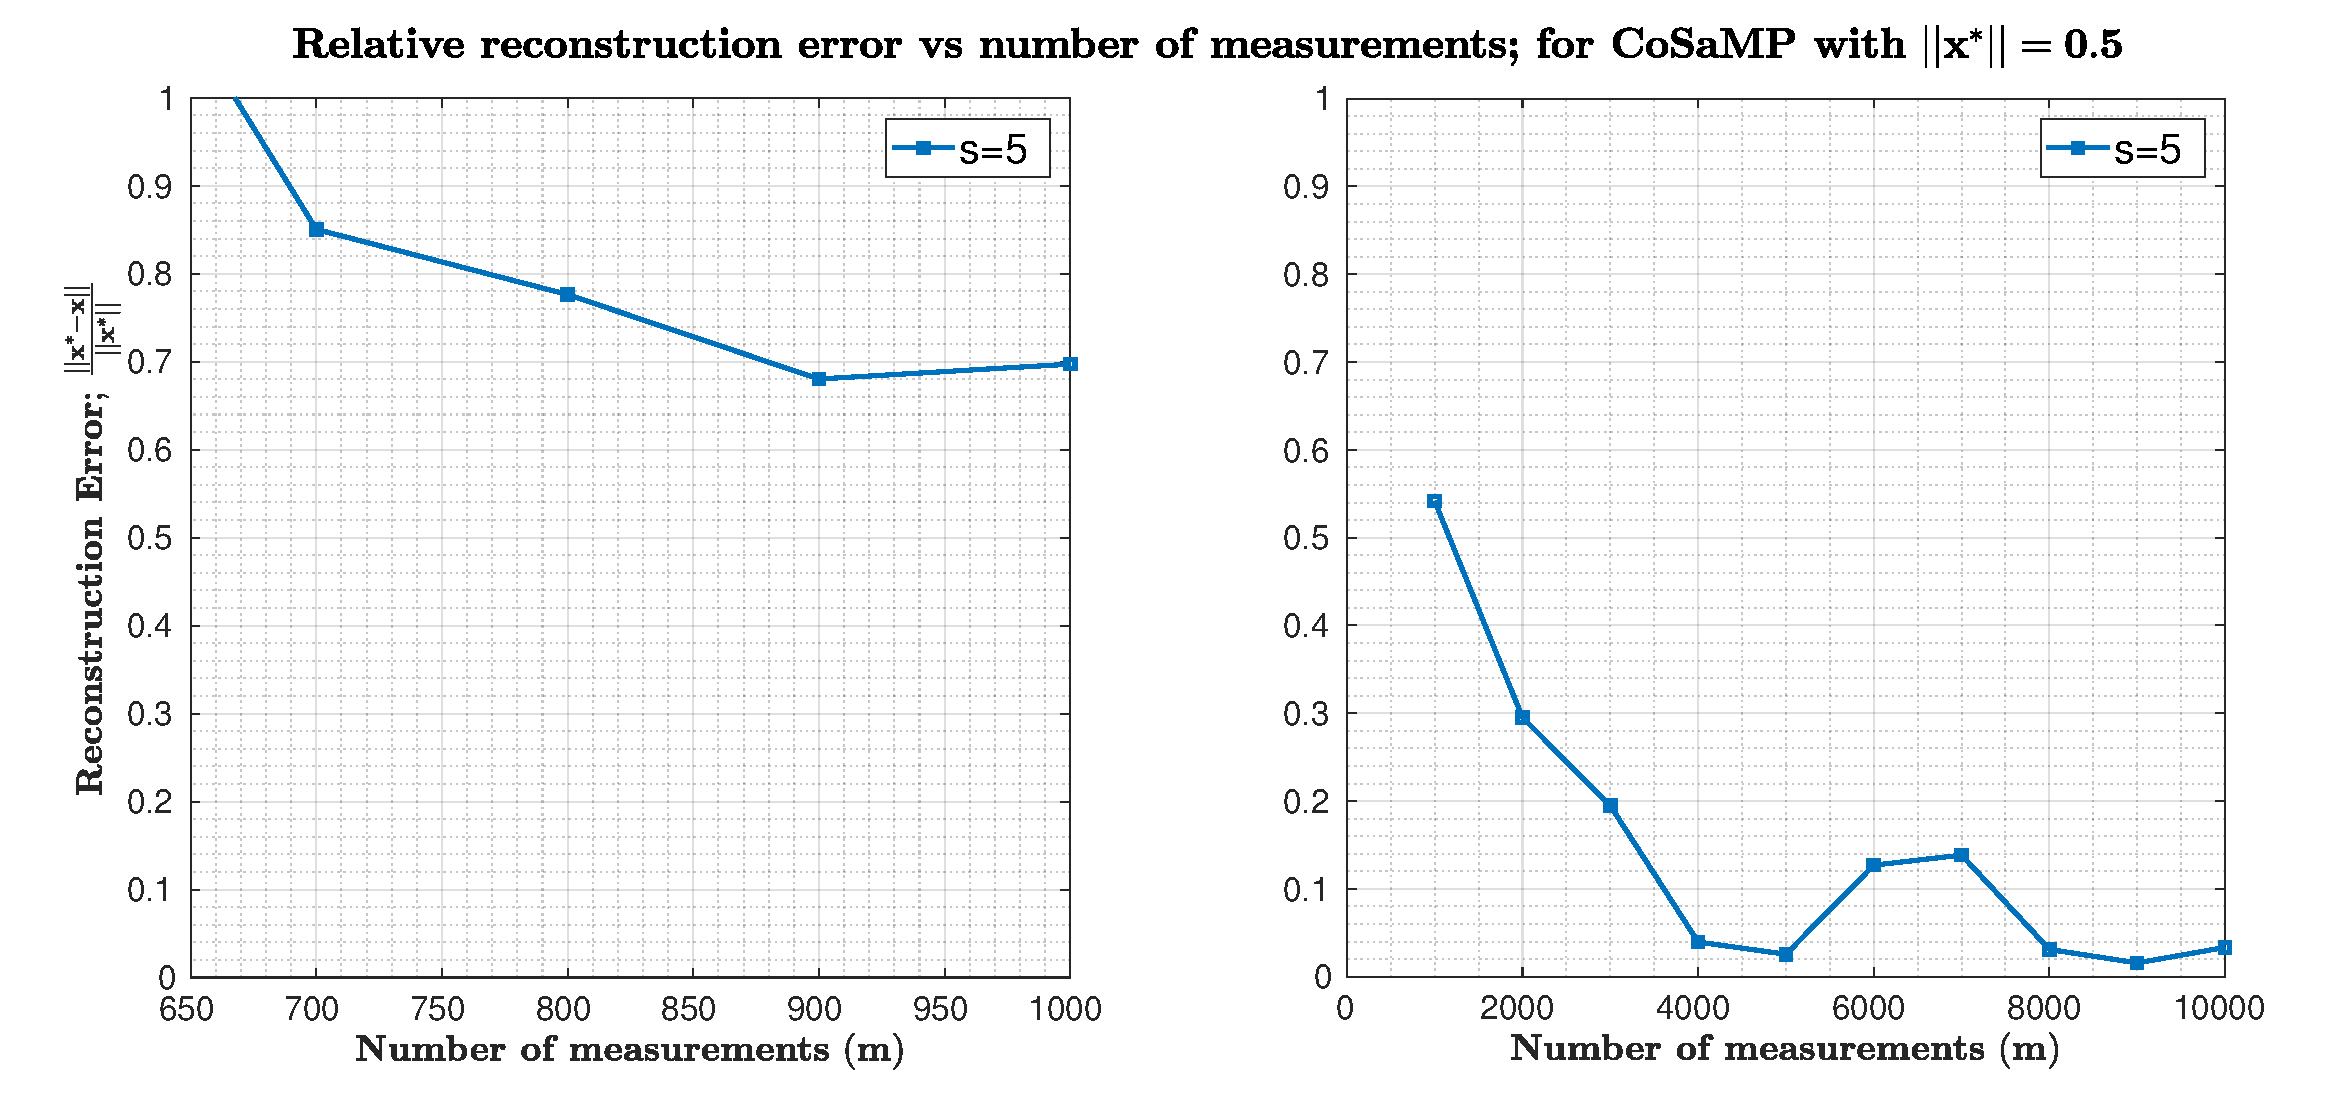
\includegraphics[width=\linewidth]{./fig/plot-1-2.pdf}
	\end{center}
	\caption{}
	\label{fig:plot-1-2}
\end{figure}
%
\begin{figure}[t]
	\begin{center}
		%\vspace{-0em}
		\includegraphics[width=\linewidth]{./fig/plot-1-3.pdf}
	\end{center}
	\caption{}
	\label{fig:plot-1-3}
\end{figure}
%
\begin{figure}[H]
	\begin{center}
		%\vspace{-0em}
		\includegraphics[width=\linewidth]{./fig/plot-1-1.pdf}
	\end{center}
	\caption{}
	\label{fig:plot-1-4}
\end{figure}
\section{Discussion}
\label{sec:disc}
In this paper, for signal recovery from compressed modulo measurements, we presented a novel algorithmic approach inspired from the classical phase retrieval solutions. Our mathematical and experimental analysis support our claim of exact signal recovery through proposed algorithm. Several open questions remain that can serve as the future directions of our work. While in this paper we considered only two periods within the modulo operation, extending the proposed approach for more periods (and theoretically infinite periods) is a significant and interesting research direction. Instead of relying on sparsity prior for compressed recovery, employing novel set of priors such as GAN priors\cite{bora2017compressed,shah2018solving} can also be a direction to be explored. Moreover, our analysis is limited to the case of Gaussian measurements, thus extending our results to various measurement schemes such as Fourier samples can be an interesting problem for future study. 
%\section{Appendix}
\label{sec:append}
%\input{./model}
%\clearpage
%\input{../common/ack}
\bibliographystyle{plain}
\bibliography{./vsbib}
%\input{../common/appendix_a}
%\input{../common/appendix_b}

\end{document}